% !TEX program = pdflatex
% !TEX root = Documentacion.tex
\documentclass[12pt,a4paper]{article}
\usepackage[utf8]{inputenc}
\usepackage{babel}
\usepackage{geometry}
\usepackage{graphicx}
\usepackage{fancyhdr}
\usepackage{xcolor}
\usepackage{float}
\usepackage{array}
\usepackage{booktabs}
\usepackage{tabularx}
\usepackage{longtable}
\usepackage{hyperref}
\usepackage{tikz}
\usetikzlibrary{arrows.meta,positioning,shapes.geometric,calc}

\geometry{margin=2.5cm}
\setlength{\headheight}{14.5pt}


% Encabezado y pie de página
\pagestyle{fancy}
\fancyhf{}
\lhead{Paradigmas de Programación}
\rhead{CE-1106}
\cfoot{\thepage}

\title{
    \textbf{Instituto Tecnológico de Costa Rica} \\
    \large Escuela de Ingeniería en Computación \\
    \large Paradigmas de Programación (CE-1106) \\
    \vspace{0.5cm}
    \Large \textbf{Implementación de juego 2048 en Racket}
}
\author{Jeremy Serracin Oporta - 2022164175
\\ Sebastián Bolaños Zamora - 2024099520
\\ Andrés Madrigal Vega - 2021572460}
\date{9 de Abril de 2026}

\begin{document}

\maketitle
\thispagestyle{empty}

\tableofcontents
\newpage

\section{Documento tecnico}

\subsection{Descripcion de las funciones implementadas}

El proyecto se divide en dos modulos principales: \texttt{Logica.rkt} (reglas del juego) y \texttt{2048.rkt}
(interfaz grafica, animaciones y ciclo de ejecucion). Esta separacion permite mantener la logica funcional
aislada de la parte visual del programa.

\subsubsection*{Funciones principales del modulo \texttt{Logica.rkt}}

\begin{longtable}{p{0.40\textwidth}p{0.50\textwidth}}
\toprule
\textbf{Funcion} & \textbf{Descripcion tecnica} \\
\midrule
\endhead
\texttt{nonzero?} & Predicado que verifica si un valor es distinto de 0. Se usa para filtrar casillas vacias. \\
\texttt{pad-right} & Rellena una lista hasta una longitud objetivo con un valor de padding (en este caso, 0). \\
\texttt{combine} & Combina pares adyacentes iguales en una fila (por ejemplo, \texttt{(2 2 4)} pasa a \texttt{(4 4)}). \\
\texttt{combine-total} & Calcula el total de puntos producidos por combinaciones en una fila, sin alterar la semantica del movimiento. \\
\texttt{slide-left} & Algoritmo base del juego: filtra ceros, combina y rellena a la derecha. \\
\texttt{slide-right} & Movimiento hacia la derecha aplicando simetria con \texttt{reverse} + \texttt{slide-left}. \\
\texttt{left}, \texttt{right}, \texttt{up}, \texttt{down} & Aplican deslizamiento sobre el tablero completo. \texttt{up/down} usan transposicion para reutilizar logica. \\
\texttt{score-increment} & Suma el puntaje ganado en una jugada a partir del tablero previo al movimiento final. \\
\texttt{moves-row-left/right} & Generan trazas de movimiento por ficha para la animacion (origen y destino). \\
\texttt{moves-grid-left/right/up/down} & Generalizan las trazas al tablero completo por direccion. \\
\texttt{chop} & Convierte la representacion lineal del estado en una matriz por filas. \\
\texttt{count-zeros} & Cuenta casillas vacias para seleccionar donde insertar una nueva ficha. \\
\texttt{index-of-nth-zero} & Ubica la posicion de la n-esima casilla vacia. \\
\texttt{replace-nth-zero} & Inserta un valor (2 o 4) en una casilla vacia especifica. \\
\texttt{new-tile} & Genera ficha nueva: 2 con 90\% de probabilidad y 4 con 10\%. \\
\texttt{initial-state} & Crea estado inicial cuadrado (lado por defecto 4). \\
\texttt{initial-state-mxn} & Crea estado inicial para tableros MxN, con validacion de rango 4 a 10. \\
\texttt{finished?} & Verifica si no existen jugadas validas en ninguna direccion. \\
\texttt{won-game?} & Verifica victoria cuando aparece la ficha objetivo \texttt{2048}. \\
\bottomrule
\end{longtable}

\subsubsection*{Funciones principales del modulo \texttt{2048.rkt}}

\begin{longtable}{p{0.40\textwidth}p{0.50\textwidth}}
\toprule
\textbf{Funcion} & \textbf{Descripcion tecnica} \\
\midrule
\endhead
\texttt{state->image} & Convierte el estado del juego a una imagen del tablero, casilla por casilla. \\
\texttt{make-tile} & Construye la ficha grafica (fondo + texto), con memoizacion para rendimiento. \\
\texttt{moves->frame} & Genera un fotograma interpolado para animar desplazamientos. \\
\texttt{animate-moving-tiles} & Produce secuencia de fotogramas para movimiento de fichas. \\
\texttt{animate-appearing-tile} & Produce secuencia de crecimiento para la ficha recien insertada. \\
\texttt{key->ops} & Traduce teclas de flecha en funciones de movimiento y trazado. \\
\texttt{change} & Funcion central de actualizacion: aplica jugada, puntaje, insercion aleatoria y cola de animaciones. \\
\texttt{show-world} & Dibuja tablero, puntaje, tiempo y mensajes de estado (victoria/derrota). \\
\texttt{advance-frame} & Consume la cola de fotogramas y avanza la animacion en cada tick. \\
\texttt{game-over?} & Determina condicion de parada: sin movimientos, victoria o limite de tiempo. \\
\texttt{parse-size}, \texttt{prompt-size} & Entrada interactiva para dimension MxN con validacion. \\
\texttt{prompt-demo-mode} & Activa modo demostracion para mostrar estado ganador inicial. \\
\texttt{start} & Punto de entrada del programa; configura \texttt{big-bang}. \\
\bottomrule
\end{longtable}

\subsection{Ejemplificacion de las estructuras de datos desarrolladas}

\subsubsection*{Estructura 1: tablero como lista lineal}
Representacion principal del estado interno:

\begin{center}
\texttt{(2 0 0 2)}
\end{center}

Para un tablero 2x2, la lista anterior corresponde a:

\begin{center}
\texttt{((2 0) (0 2))}
\end{center}

Esta conversion se realiza con la funcion \texttt{chop}, que agrupa la lista lineal en sublistas por filas.

\subsubsection*{Estructura 2: tablero matricial (lista de listas)}
Usado para aplicar movimientos por fila o por columna:

\begin{center}
\texttt{((2 0 2 4) (0 4 0 4) (2 2 0 0) (0 0 0 2))}
\end{center}

Cada sublista representa una fila del tablero.

\subsubsection*{Estructura 3: registro de movimiento para animacion}
Cada movimiento individual se modela como:

\begin{center}
\texttt{(valor (fila-origen col-origen) (fila-destino col-destino))}
\end{center}

Ejemplo:

\begin{center}
\texttt{(2 (0 1) (0 0))}
\end{center}

Significa: la ficha 2 se mueve de la posicion (0,1) a la posicion (0,0).

\subsubsection*{Estructura 4: estado global del mundo (struct \texttt{world})}
La estructura del juego en ejecucion contiene:

\begin{center}
\texttt{(world state score winning-total rows cols frames start-time)}
\end{center}

Campos:
\begin{itemize}
    \item \texttt{state}: tablero lineal.
    \item \texttt{score}: puntaje acumulado.
    \item \texttt{winning-total}: valor objetivo para detectar estado ganador en demo.
    \item \texttt{rows}, \texttt{cols}: dimensiones del tablero.
    \item \texttt{frames}: cola de funciones de render para animaciones.
    \item \texttt{start-time}: marca temporal de inicio.
\end{itemize}

\subsubsection*{Estructura 5: tablas de mapeo para estilos graficos}
Se utilizan listas asociativas para definir colores de fondo y texto por valor de ficha:

\begin{center}
\texttt{((2 colorA) (4 colorB) (8 colorC) ...)}
\end{center}

Esto simplifica la personalizacion visual y evita condicionales extensos.

\subsection{Descripcion detallada de los algoritmos desarrollados}

\subsubsection*{Algoritmo A: deslizamiento y combinacion hacia la izquierda}
\textbf{Objetivo:} aplicar las reglas base de 2048 en una fila.

\textbf{Pasos:}
\begin{enumerate}
    \item Filtrar ceros (casillas vacias).
    \item Recorrer y combinar pares adyacentes iguales una sola vez por turno.
    \item Rellenar con ceros hasta recuperar la longitud original.
\end{enumerate}

\textbf{Ejemplo:}
\begin{center}
\texttt{(2 0 2 4) -> (2 2 4) -> (4 4) -> (4 4 0 0)}
\end{center}

\textbf{Complejidad:} O(n) por fila.

\begin{figure}[H]
    \centering
    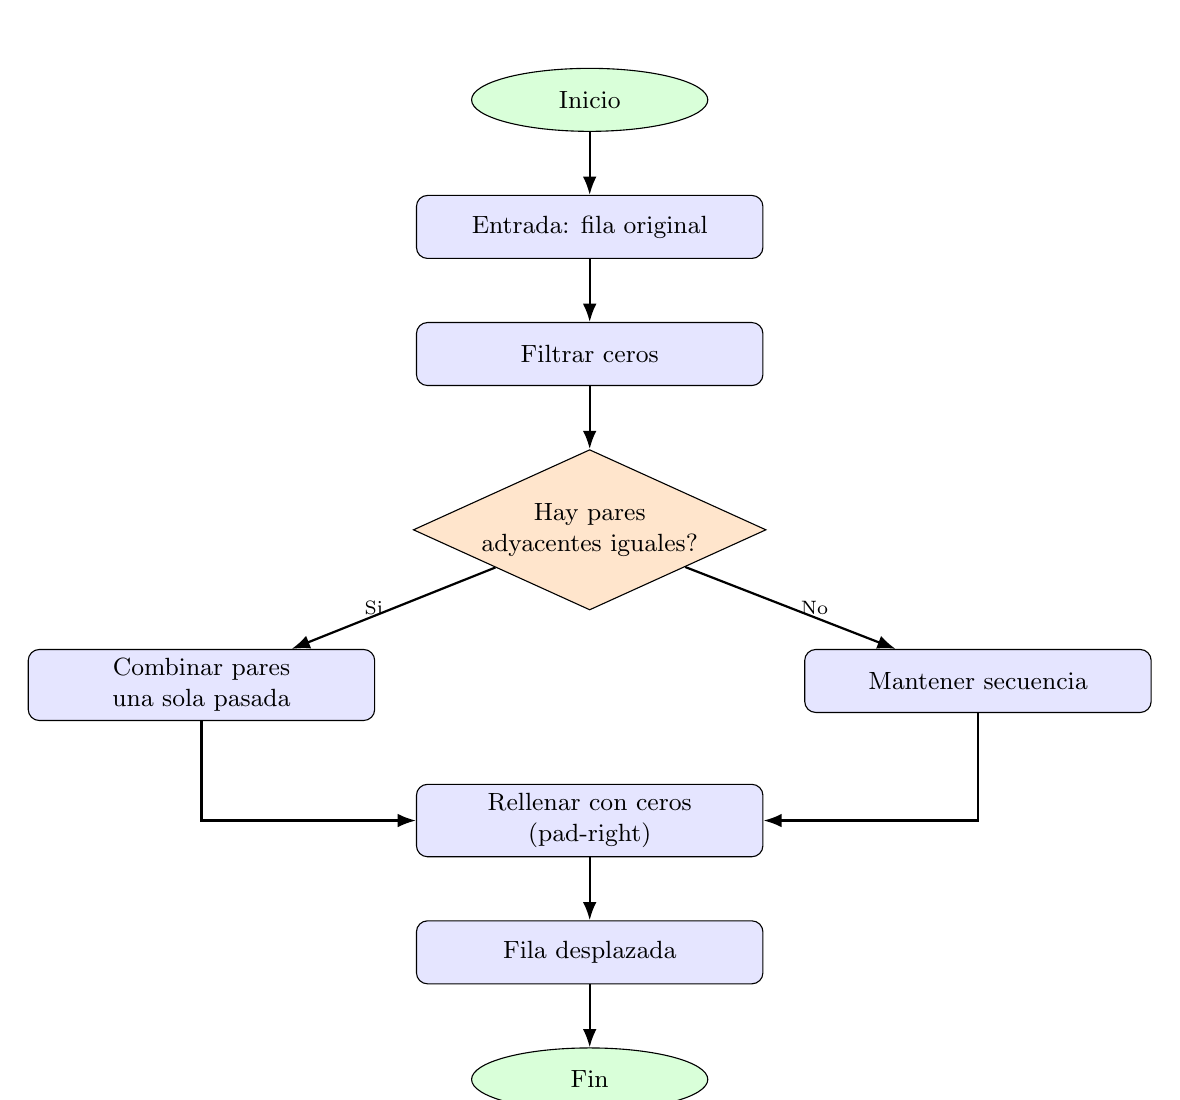
\begin{tikzpicture}[
        >=Latex,
        node distance=8mm and 14mm,
        startstop/.style={ellipse, draw=black, fill=green!15, align=center, minimum width=30mm, minimum height=8mm, font=\small},
        process/.style={rectangle, rounded corners, draw=black, fill=blue!10, align=center, minimum width=44mm, minimum height=8mm, font=\small},
        decision/.style={diamond, draw=black, fill=orange!20, align=center, aspect=2.2, inner sep=1.2pt, font=\small},
        arrow/.style={->, thick}
    ]
        \node[startstop] (start) {Inicio};
        \node[process, below=of start] (input) {Entrada: fila original};
        \node[process, below=of input] (filter) {Filtrar ceros};
        \node[decision, below=of filter] (pairs) {Hay pares\\adyacentes iguales?};
        \node[process, below left=10mm and 16mm of pairs] (combine) {Combinar pares\\una sola pasada};
        \node[process, below right=10mm and 16mm of pairs] (skip) {Mantener secuencia};
        \node[process, below=22mm of pairs] (pad) {Rellenar con ceros\\(pad-right)};
        \node[process, below=of pad] (output) {Fila desplazada};
        \node[startstop, below=of output] (end) {Fin};

        \draw[arrow] (start) -- (input);
        \draw[arrow] (input) -- (filter);
        \draw[arrow] (filter) -- (pairs);
        \draw[arrow] (pairs) -- node[left, font=\scriptsize] {Si} (combine);
        \draw[arrow] (pairs) -- node[right, font=\scriptsize] {No} (skip);
        \draw[arrow] (combine) |- (pad);
        \draw[arrow] (skip) |- (pad);
        \draw[arrow] (pad) -- (output);
        \draw[arrow] (output) -- (end);
    \end{tikzpicture}
    \caption{Diagrama del algoritmo de deslizamiento hacia la izquierda.}
\end{figure}

\subsubsection*{Algoritmo B: movimientos en las cuatro direcciones}
\textbf{Objetivo:} reutilizar logica para evitar duplicacion de codigo.

\textbf{Idea principal:}
\begin{itemize}
    \item \texttt{left}: aplica \texttt{slide-left} a cada fila.
    \item \texttt{right}: invierte fila, aplica \texttt{slide-left}, reinvierte.
    \item \texttt{up/down}: transpone tablero, aplica izquierda/derecha y vuelve a transponer.
\end{itemize}

\textbf{Complejidad:} O(MxN) por movimiento completo del tablero.

\begin{figure}[H]
    \centering
    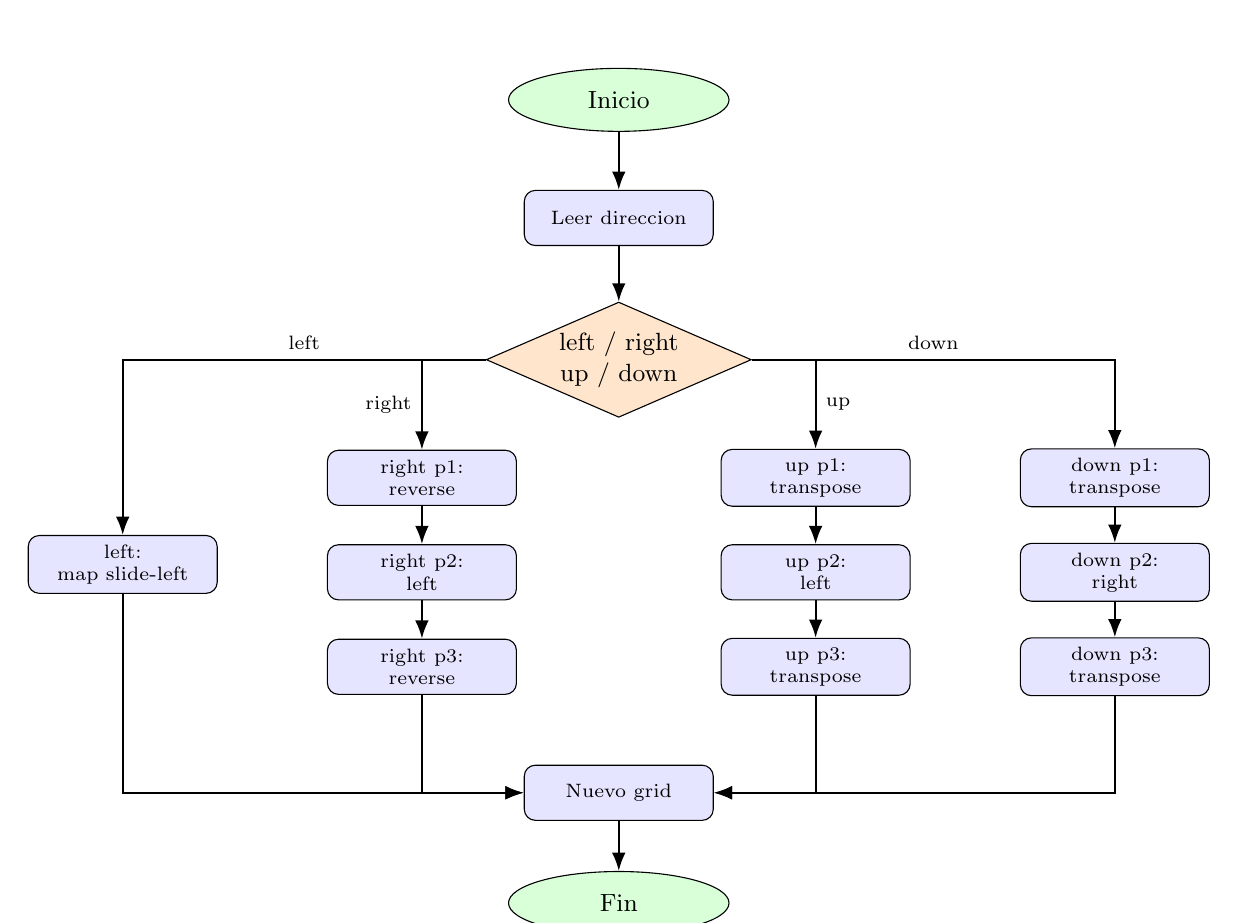
\begin{tikzpicture}[
            >=Latex,
            startstop/.style={ellipse, draw=black, fill=green!15, align=center, minimum width=28mm, minimum height=8mm, font=\small},
            process/.style={rectangle, rounded corners, draw=black, fill=blue!10, align=center, minimum width=24mm, minimum height=7mm, font=\scriptsize},
            decision/.style={diamond, draw=black, fill=orange!20, align=center, aspect=2.3, inner sep=1pt, font=\small},
            arrow/.style={->, thick}
        ]
        \node[startstop] (start) at (0,0) {Inicio};
        \node[process] (read) at (0,-1.5) {Leer direccion};
        \node[decision] (choose) at (0,-3.3) {left / right\\up / down};
        \node[process] (leftn) at (-6.3,-5.9) {left:\\map slide-left};
        \node[process] (r1) at (-2.5,-4.8) {right p1:\\reverse};
        \node[process] (r2) at (-2.5,-6.0) {right p2:\\left};
        \node[process] (r3) at (-2.5,-7.2) {right p3:\\reverse};
        \node[process] (u1) at (2.5,-4.8) {up p1:\\transpose};
        \node[process] (u2) at (2.5,-6.0) {up p2:\\left};
        \node[process] (u3) at (2.5,-7.2) {up p3:\\transpose};
        \node[process] (d1) at (6.3,-4.8) {down p1:\\transpose};
        \node[process] (d2) at (6.3,-6.0) {down p2:\\right};
        \node[process] (d3) at (6.3,-7.2) {down p3:\\transpose};
        \node[process] (merge) at (0,-8.8) {Nuevo grid};
        \node[startstop] (end) at (0,-10.2) {Fin};

        \draw[arrow] (start) -- (read);
        \draw[arrow] (read) -- (choose);

        \draw[arrow] (choose.west) -| node[pos=0.25, above, font=\scriptsize] {left} (leftn.north);

        
        \draw[arrow] (choose.west -| r1) -- node[left, font=\scriptsize] {right} (r1.north);

        
        \draw[arrow] (choose.east -| u1) -- node[right, font=\scriptsize] {up} (u1.north);

        
        \draw[arrow] (choose.east) -| node[pos=0.25, above, font=\scriptsize] {down} (d1.north);

        \draw[arrow] (r1) -- (r2);
        \draw[arrow] (r2) -- (r3);
        \draw[arrow] (u1) -- (u2);
        \draw[arrow] (u2) -- (u3);
        \draw[arrow] (d1) -- (d2);
        \draw[arrow] (d2) -- (d3);
        \draw[arrow] (leftn) |- (merge);
        \draw[arrow] (r3) |- (merge);
        \draw[arrow] (u3) |- (merge);
        \draw[arrow] (d3) |- (merge);
        \draw[arrow] (merge) -- (end);
    \end{tikzpicture}
    \caption{Diagrama de flujo del movimiento por direccion.}
\end{figure}

\subsubsection*{Algoritmo C: calculo de puntaje}
\textbf{Objetivo:} sumar el valor de las combinaciones realizadas en cada turno.

\textbf{Pasos:}
\begin{enumerate}
    \item Para cada fila, obtener solo fichas no vacias.
    \item Calcular total de combinaciones con \texttt{combine-total}.
    \item Sumar resultados de todas las filas.
\end{enumerate}

\textbf{Complejidad:} O(MxN).

\subsubsection*{Algoritmo D: insercion aleatoria de nueva ficha}
\textbf{Objetivo:} simular generacion de nueva ficha despues de una jugada valida.

\textbf{Pasos:}
\begin{enumerate}
    \item Contar cantidad de ceros en el estado.
    \item Elegir una posicion vacia aleatoria.
    \item Generar valor con distribucion: 90\% de 2, 10\% de 4.
    \item Reemplazar la casilla vacia seleccionada.
\end{enumerate}

\textbf{Complejidad:} O(MxN) por busqueda y reemplazo.

\subsubsection*{Algoritmo E: deteccion de fin de juego y victoria}
\textbf{Objetivo:} decidir si la partida debe continuar o finalizar.

\textbf{Reglas:}
\begin{itemize}
    \item \textbf{Fin por bloqueo:} no hay cambios al intentar mover en ninguna direccion.
    \item \textbf{Fin por victoria:} se alcanza ficha objetivo (2048).
\end{itemize}

\subsubsection*{Algoritmo F: pipeline de animacion}
\textbf{Objetivo:} ofrecer transiciones visuales suaves entre estados.

\textbf{Pipeline:}
\begin{enumerate}
    \item Generar 9 fotogramas de desplazamiento (interpolacion lineal).
    \item Generar 4 fotogramas de aparicion de ficha nueva (escalado progresivo).
    \item Encolar los fotogramas como funciones en \texttt{frames}.
    \item Consumir un frame por tick de \texttt{big-bang}.
\end{enumerate}

\begin{figure}[H]
    \centering
    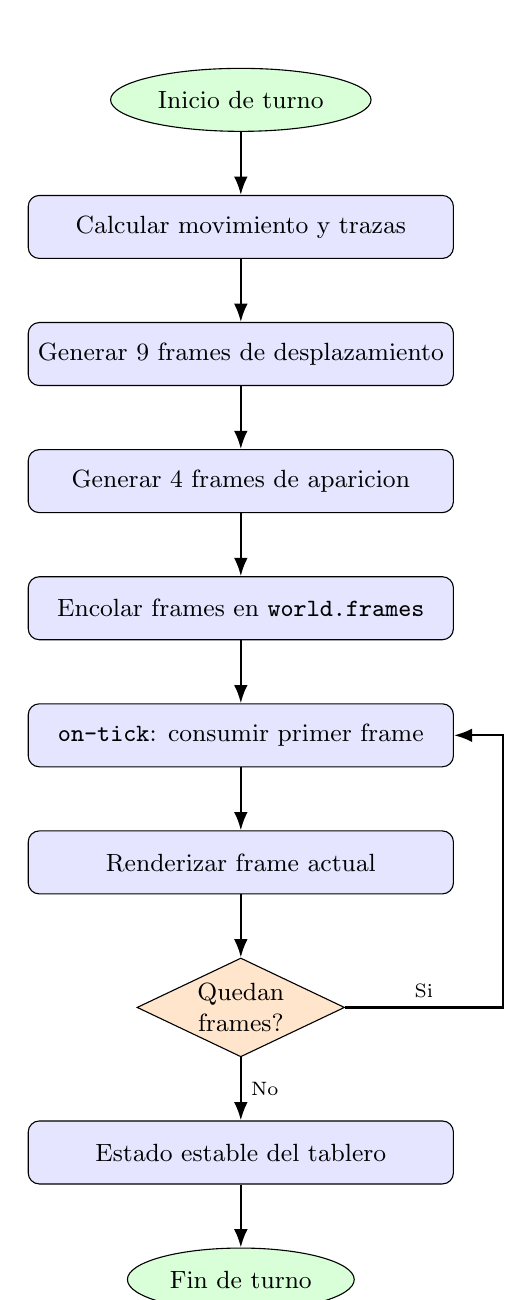
\begin{tikzpicture}[
        >=Latex,
        node distance=8mm and 12mm,
        startstop/.style={ellipse, draw=black, fill=green!15, align=center, minimum width=28mm, minimum height=8mm, font=\small},
        process/.style={rectangle, rounded corners, draw=black, fill=blue!10, align=center, minimum width=54mm, minimum height=8mm, font=\small},
        decision/.style={diamond, draw=black, fill=orange!20, align=center, aspect=2.1, inner sep=1.2pt, font=\small},
        arrow/.style={->, thick}
    ]
        \node[startstop] (start) {Inicio de turno};
        \node[process, below=of start] (move) {Calcular movimiento y trazas};
        \node[process, below=of move] (frames1) {Generar 9 frames de desplazamiento};
        \node[process, below=of frames1] (frames2) {Generar 4 frames de aparicion};
        \node[process, below=of frames2] (queue) {Encolar frames en \texttt{world.frames}};
        \node[process, below=of queue] (tick) {\texttt{on-tick}: consumir primer frame};
        \node[process, below=of tick] (render) {Renderizar frame actual};
        \node[decision, below=of render] (more) {Quedan\\frames?};
        \node[process, below=of more] (stable) {Estado estable del tablero};
        \node[startstop, below=of stable] (end) {Fin de turno};

        \draw[arrow] (start) -- (move);
        \draw[arrow] (move) -- (frames1);
        \draw[arrow] (frames1) -- (frames2);
        \draw[arrow] (frames2) -- (queue);
        \draw[arrow] (queue) -- (tick);
        \draw[arrow] (tick) -- (render);
        \draw[arrow] (render) -- (more);
        \draw[arrow] (more) -- node[right, font=\scriptsize] {No} (stable);
        \draw[arrow] (stable) -- (end);

        \draw[arrow] (more.east) -- ++(20mm,0) node[midway, above, font=\scriptsize] {Si} |- (tick.east);
    \end{tikzpicture}
    \caption{Pipeline de animacion del estado del juego.}
\end{figure}

\subsection{Problemas sin solucion}

Los siguientes puntos fueron identificados como mejoras potenciales que no se resolvieron en esta entrega:

\begin{enumerate}
    \item \textbf{Persistencia de partida}: no existe guardado/carga del estado del juego.
    \item \textbf{Historial de jugadas (undo)}: no se implemento deshacer movimiento.
    \item \textbf{Escalabilidad visual}: para tableros muy grandes (10x10) la legibilidad se reduce por limites de tamano de ventana.
\end{enumerate}

\subsection{Plan de actividades realizadas por estudiante}

La Tabla~\ref{tab:plan} presenta un plan de trabajo editable con descripcion de tarea, tiempo estimado,
fecha de entrega y responsable.

\begin{table}[H]
\centering
\caption{Plan de actividades por estudiante}
\label{tab:plan}
\begin{tabularx}{\textwidth}{>{\raggedright\arraybackslash}p{0.2\textwidth} >{\raggedright\arraybackslash}p{0.35\textwidth} >{\centering\arraybackslash}p{0.12\textwidth} >{\centering\arraybackslash}p{0.15\textwidth} }
\toprule
\textbf{Estudiante} & \textbf{Actividad} & \textbf{Tiempo est.} & \textbf{Fecha entrega} \\
\midrule

Sebastián Bolaños Zamora & Implementacion de reglas de deslizamiento, combinacion y puntaje. & 10 h & 26/03/2026 \\
Andrés Madrigal Vega & Diseño de interfaz grafica, animaciones y ciclo \texttt{big-bang}. & 9 h & 05/04/2026 \\
Jeremy Serracin Oporta & Validacion de entrada MxN, pruebas manuales, documentacion tecnica, manual de usuario y generacion de ejecutable. & 7 h & 08/04/2026 \\

\bottomrule
\end{tabularx}
\end{table}

\subsection{Problemas encontrados}

\subsubsection*{Problema 1: combinaciones consecutivas incorrectas en una fila}
\textbf{Descripcion detallada:} en pruebas tempranas, una fila con patron repetido podia producir resultados no esperados si la combinacion
no respetaba la regla de \textit{una fusion por ficha y por turno}.

\textbf{Intentos de solucion sin exito:}
\begin{itemize}
    \item Aplicar combinaciones en multiples pasadas sobre la misma fila.
    \item Combinar antes de eliminar ceros, lo cual alteraba el orden real de desplazamiento.
\end{itemize}

\textbf{Solucion encontrada:}
se establecio el orden correcto del algoritmo: filtrar ceros, combinar una sola pasada de izquierda a derecha,
y luego rellenar con ceros. Esta estrategia se formalizo con \texttt{slide-left} y \texttt{combine}.

\textbf{Recomendaciones:}
agregar baterias de pruebas de filas con patrones limite: \texttt{(2 2 2 2)}, \texttt{(4 0 4 4)}, \texttt{(0 2 0 2)}.

\textbf{Conclusion del problema:}
la correccion del orden de transformacion estabilizo tanto el movimiento como el puntaje acumulado.

\textbf{Bibliografia especifica del problema:}
[1], [2], [3].

\subsubsection*{Problema 2: desincronizacion visual entre estado y animacion}
\textbf{Descripcion detallada:} al actualizar estado y dibujar inmediatamente, algunas fichas aparecian en su posicion final
sin mostrar desplazamiento suave.

\textbf{Intentos de solucion sin exito:}
\begin{itemize}
    \item Redibujar el estado final en cada tick sin interpolacion.
    \item Reducir intervalo de tick sin cola de fotogramas.
\end{itemize}

\textbf{Solucion encontrada:}
se introdujo una cola de \texttt{frames} (funciones sin argumentos) y dos fases de animacion:
desplazamiento interpolado y aparicion escalada de la nueva ficha.

\textbf{Recomendaciones:}
parametrizar cantidad de frames para adaptar fluidez segun tamano de tablero y rendimiento del equipo.

\textbf{Conclusion del problema:}
la animacion en dos fases mejora la claridad visual de cada jugada y la experiencia de usuario.

\textbf{Bibliografia especifica del problema:}
[4], [5].

\subsection{Conclusiones y recomendaciones del proyecto}

\textbf{Conclusiones:}
\begin{itemize}
    \item Se logro una implementacion funcional de 2048 en Racket con separacion clara entre logica y visualizacion.
    \item El enfoque funcional simplifico la verificacion de reglas del juego y redujo efectos secundarios en el modulo logico.
    \item La arquitectura basada en \texttt{big-bang} permitio integrar entrada, animacion y renderizado de forma consistente.
\end{itemize}

\textbf{Recomendaciones:}
\begin{itemize}
    \item Incorporar pruebas automatizadas por casos de combinacion para prevenir regresiones.
    \item Implementar historial de jugadas para modo \textit{undo} y soporte de depuracion.
    \item Mejorar escalado visual adaptativo para tableros de mayor tamano.
    \item Agregar persistencia de partida para mejorar continuidad de uso.
\end{itemize}

\subsection{Bibliografia consultada en todo el proyecto}

\begin{enumerate}
    \item Racket Documentation, \textit{The Racket Guide}. [En linea]. Disponible en: \url{https://docs.racket-lang.org/guide/}
    \item Racket Documentation, \textit{The Racket Reference}. [En linea]. Disponible en: \url{https://docs.racket-lang.org/reference/}
    \item Racket Documentation, \textit{2htdp/universe: World Programs}. [En linea]. Disponible en: \url{https://docs.racket-lang.org/teachpack/2htdpuniverse.html}
    \item Racket Documentation, \textit{2htdp/image: Image Library}. [En linea]. Disponible en: \url{https://docs.racket-lang.org/teachpack/2htdpimage.html}
    \item G. Helser, \textit{How to Design Programs, 2nd ed.}, MIT Press, 2018.
\end{enumerate}

\end{document}